\documentclass[english, a4paper, 12pt, twoside]{book}

% -------------- Setup, do not change these ---------------
\usepackage{textcomp}
\usepackage[T1]{fontenc, url}
\usepackage[utf8]{inputenc}
\usepackage{titlesec}
\setcounter{secnumdepth}{4}
\usepackage{multirow}
\usepackage{braket}


\usepackage{adjustbox}
\usepackage{graphicx}
\usepackage{amsmath, amssymb, amsthm} % Mathematical packages
\usepackage{parskip} % Removing indenting in new paragraphs
\urlstyle{sf}
\usepackage{color}
\usepackage{subcaption}
\usepackage{appendix}
\usepackage{chngcntr} % needed for correct table numbering
\counterwithin{table}{section} % numbering of tables
\counterwithin{figure}{section} % numbering of figures
\numberwithin{equation}{section} % numbering of equations
\hyphenpenalty=100000 % preventing splitting of words
\sloppy
\raggedbottom
\usepackage{xparse,nameref}
\usepackage[bottom]{footmisc} % Fotnotes are fixed to bottom of page

% --------- You can edit from this point on --------


% ----- Appearance and language -----
\usepackage[english]{babel} % document language
\graphicspath{./img/} % path to images
\usepackage[margin=2.54cm]{geometry} % sets margins for the document
\usepackage{setspace}
\linespread{1} % line spread for the document
\usepackage{microtype}


% ----- Sections -----
\titleformat*{\section}{\LARGE\bfseries} % \section heading
\titleformat*{\subsection}{\Large\bfseries} % \subsection heading
\titleformat*{\subsubsection}{\large\bfseries} % \subsubsection heading
% next three lines creates the \paragraph command with correct heading
\titleformat{\paragraph}
{\normalfont\normalsize\bfseries}{\theparagraph}{1em}{}
\titlespacing*{\paragraph}
{0pt}{3.25ex plus 1ex minus .2ex}{1.5ex plus .2ex}


% ----- Figures and tables -----
\usepackage{fancyhdr}
\usepackage{subfiles}
\usepackage{array}
\usepackage[rightcaption]{sidecap}
\usepackage{wrapfig}
\usepackage{float}
\usepackage[labelfont=bf]{caption} % bold text for captions
\usepackage[para]{threeparttable} % fancy tables, check these before you use them
\usepackage{url}
\usepackage[table,xcdraw]{xcolor}
\usepackage{makecell}
\usepackage{hhline}

\usepackage[breaklinks=true,colorlinks=true,linkcolor=black,urlcolor=blue,citecolor=blue]{hyperref}
% ----- Sources -----

%\bibliographystyle{apa} % citation and reference list style
%\def\biblio{\clearpage\bibliographystyle{apa}\bibliography{References.bib}} % defines the \biblio command used for referencing in subfiles - DO NOT CHANGE


% ----- Header and footer -----
\pagestyle{fancy}
\fancyhead[RO,LE]{\thepage} % page number on right for odd pages and left for even pages in the header
\fancyhead[RE,LO]{\nouppercase{\rightmark}} % chapter name and number on the right for even pages and left for odd pages in the header
%\renewcommand{\headrulewidth}{0pt} % sets thickness of header line
\fancyfoot{} % removes page number on bottom of page


% ----- Header of the frontpage -----
\fancypagestyle{frontpage}{
	\fancyhf{}
	\renewcommand{\headrulewidth}{0pt}
	\renewcommand{\footrulewidth}{0pt}
	\vspace*{1\baselineskip}

	%\fancyhead[R]{Norwegian School of Economics
	%\linebreak       Bergen, Fall 2018\vspace*{5\baselineskip}}
	\fancyhead[C]{ 
\includegraphics[width=3.5in]{img/logo}}
}


% ----- Document starts here -----
\begin{document}

%\def\biblio{} % resets the biblio command, if not here a new reference list will be produced after every chapter
{\setstretch{1.5}

\begin{titlepage}

 \newgeometry{top=1 in, bottom=1 in, left=1 in, right= 1 in}

 \thispagestyle{frontpage}

 \begin{center}

   \vspace*{6\baselineskip}


   {\Huge \textbf{Fancy title with many fancy words\\}}

   

       \vspace*{1,5\baselineskip}


   \vspace{1,5\baselineskip}

   \large{A master’s thesis submitted to the faculty of mathematics, computer science and physics, of the University of Innsbruck\\ in partial fulfillment of the requirements for the degree of\\\vspace{1,2\baselineskip}\textbf{Master of Science (MSc)} \\\vspace{1,2\baselineskip}carried out at the Institute of Experimental Physics under the supervision of}\\
   \large{o.Univ.-Prof.  Dr.  Rainer Blatt,}\\
   \large{Dr. Ben Lanyon}\\
    \vspace{1,2\baselineskip}
   \large{Presented by\\}
   \huge{\textbf{Marco Canteri}}\\
   

 \end{center}

\end{titlepage}

}
\restoregeometry % restores the margins after frontpage
%\nocite{*} % uncomment if you want all sources to be printed in the reference list, including the ones which are not cited in the text

\pagenumbering{gobble} % suppress page numbering
\thispagestyle{plain} % suppress header
\clearpage\mbox{}\clearpage % add blank page

\pagenumbering{roman} % starting roman page numbering
\newpage

\section*{Abstract}
I swear I did something

\newpage


\newpage
\tableofcontents

\newpage
\listoffigures

\newpage
\addtocontents{toc}{\protect\setcounter{tocdepth}{4}} % sets depth of toc to 4, 1.1.1.1
\pagenumbering{arabic} % Starting arabic page numbering
\setcounter{page}{1} % sets pagecounter to 1

\chapter{Introduction} % section/chapter name

- Quantum computing/quantum networking \\
- Experiment context\\
- Master thesis project\\
- Outline\\
\newline

Quantum computing has been a rapidly increasing field of interest, which is probably due to the fact that it represents the
next step in technology advancement. Classical computers are limited in solving some particular problems that have been showed to scale exponentially, and the
\\
Due to the incredible delicate nature of qubits, they are subject to decoherence which harms the successfulness and computational power of quantum computers. Therefore scaling the number of qubit has been proven to be a difficult engineeristic challenge. Several solutions are possible: the number of qubits can scale; the dimension of qubits can decrease; or qubits can be linked together. The last solution is the approach at the base of quantum networks. The idea is to connected several quantum computers to create a cluster of nodes that can work jointly. The task of building a quantum network is not trivial, there are fundamental difference with a classical link. Although the mean can be the same, such as optical fiber, a quantum network must have the ability to distribute entanglement over it. In addition to scaling quantum computers, quantum networks allow for more secure transmission of information [], and improve measurements [?].\\
It is in this context that this thesis arises. Currently there is an ongoing project of building a three node quantum network between two buildings on the campus of the University of Innsbruck. The third node is located in IQOQI, where the thesis took place. Here an ion trap is used as node of the network and it is connected with a 400m fiber link. The 393nm lasers is responsible for the generation of the transmitted photons via a cavity enhanced Raman process. At the time of this thesis' start, the 393nm laser was shining in the whole trap. In this case, if an ion string were to be loaded, the light would hit all the ions equally and there would be no  over the single ion-photon pair. This limits the experiments and the production of photons to one single ion.\\
To overcome this limitation, an optical setup for the 393nm laser had to be built with the purpose of focusing the light to a single ion in a string. Moreover the setup should have the ability to steer the beam and focus it on a different ion. The goal of this thesis was indeed to design and build such a system. The setup is per se not complex, but the design is critical, ions separation is typical in the order of $\mu$m, which means the light should be focused down to $1-2\,\mu$m, at the limits of the optical elements involved. The steering part is simply achieved with an acousto-optical deflector (AOD), such device deflects the laser light proportionally to the applied input frequency allowing to control remotely the beam ponting of the system.\\
 Once completed, the system will allow to manipulate single ions in a string. The same laser can manipulate ions in two different ways: we already mentioned the most important, the triggering of the photon's generation; but, by driving in the laser in a different regime, it is also possible to implement a single qubit gate, namely the quantum phase shift gate []. This is used to implement quantum operations that are the base for some experiments. For instance, the characterization and beam shape probing experiment performed in this thesis is built on top of such quantum operation.\\
 \newline
 This work is presented in the following way: Chapter 2 is devoted to the theoretical background necessary to understand the rest of the work. Here the foundations of quantum computing and networking are laid down, along with the basic concepts of ion trapping; Chapter 3 presents the existing experimental setup, i.e. the already built and working blocks of the experiment where the setup designed in this thesis has been added; Chapter 4 is the core of the thesis, here the final design made with the software Zemax and simulations of different aspects of the project are introduced and presented;
Chapter 5 contains all the experimental results obtained. It is divided in two parts: First, the setup was built on a spare optical table, here we had the freedom to test the performance of the system under different aspects and decide whether or not it was satisfactory. After having the certainty that the system will work, the setup was transferred and aligned on the real experiment where limited access did not consent for easy performance testing. Here, different and more complicated experimental methods had to be used to check if the system was working properly. The description and discussion of these results are in the second part of chapter 5.

\chapter{Theoretical framework}
Quantum computing is based on a general framework that does not depend on the physical platform. Here, important concept such as qubit, and quantum operations are described before showing how we can realize them, from a theoretical point of view, with trapped ions. The same goes with quantum networking, the concept and the realization can be treated separately and they will be described in this chapter. Furthermore, in this chapter we will take a look into Gaussian beams and their properties. Since that is the shape emitted by laser, it is important to understand their characteristic and how to manipulate them. Lastly Acousto-optical interactions are introduced and studied to give an idea of how AODs work and how they can be used to steer a laser beam.
\section{Quantum logic with trapped ions}
\subsection{Quantum computer and quantum gates}
The concepts of quantum computing are borrowed and extended from classical computational theory. In the classical case, information is represented in terms of binary digits, the so called bit, essentially mapping information to a base-2 number. Information processing is done with gates acting of those numbers. The idea of quantum computer is still to encode information in a binary form, but due to the nature of quantum mechanics, a quantum bit (in short qubit) gains new features that can be exploited to perform different kind of operations that in some cases are a speed up compared to the classical case.\\
A qubit is formally any wave function that can be written as superposition of two states indicated generally with $\ket{0}$ and $\ket{1}$:
\begin{equation}
\ket{\psi} = \alpha \ket{0} + \beta\ket{1},
\end{equation}
where $\alpha,\beta$ are two complex numbers that satisfy the relationship $|\alpha|^2+|\beta|^2 = 1$.



- Qubit\\
- Quantum operations\\
\subsection{Ion qubits and laser-ion interactions}
- 2 level atom scheme\\
- Model of laser-ion interaction: rabi flops, AC stark shift
\section{Quantum networking with trapped ions}
\subsection{General introduction}
- Nodes, interface, link, protocols\\
- logic, memory, interface, Bell pairs, purification, multi-mode
- Distributed entanglement
\subsection{Cavity QED}
- Simple model atom in cavity: g,gamma, k
\section{Basics of ion trapping}
\subsection{Linear Paul trap}
- How a Paul trap works\\
- micromotion?
\subsection{Ion strings}
We have seen that the potential inside the trap can be described as an harmonic potential. It is then possible to calculate the ion separation between $N$ ion loaded in the trap. This will give us an idea of how narrowly the beam should be focused and will set an appropriate problem spatial scale.\\
We will consider only the $z$ direction where the ions are weakly confined and will form a string. The harmonic potential is then given by
\begin{equation}
V = \sum_{i=0}^N \frac{1}{2}M\omega^2z_i^2 + \sum_{i\neq j}^N\frac{Z^2e^2}{8\pi \epsilon_0}\frac{1}{|z_i-z_j|}
\end{equation}
The equilibrium position can be found at the minima of the potential, i.e. where the first derivative zeros
\begin{equation}
\frac{\partial V}{\partial z_i} = 0 \implies u_i - \sum_{j=1}^{i-1} \frac{1}{(u_i-u_j)^2} + \sum_{j= i+1}^{N} \frac{1}{(u_i-u_j)^2}= 0,
\end{equation}
where we defined the dimensionless quantity $u_i = z_i/l$ and $l^3 = \displaystyle\frac{Z^2 e^2 }{4\pi \epsilon_0 M\omega^2}$.
The last equations can be solved analytically only for 2 or 3 ions. In fact, for the case $N=2$ we simply get the system
\begin{equation}
\begin{cases}
  u_1 + \frac{1}{(u_1-u_2)^2} = 0\\
  u_2 - \frac{1}{(u_1-u_2)^2} = 0
  \end{cases} \quad \implies \quad u_1 = -u_2,\quad  u_1 = \left(\frac{1}{2}\right)^{2/3} \simeq 0.629
\end{equation}
For calcium-40 ions in a Paul trap with axial confinement of 1MHz, we have $l \simeq 4.45\times 10^{-6}\, \mu$m, which means that 2 ions are separated by $\simeq 5.6\, \mu$m. In the case of more ions the separation is lesser with the same confinement, but it is also possible to lower the axial frequency and increase the separation between the ions such that also in the case of several ions, the distance between them is still in the order of several $\mu$m. This size is accessible with current focusing optics and it is above the diffraction limit.\\
For more ions, a numerical approach has to be used, \cite{ion_spacing} reports values of $u_i$ up to $N=10$, and gives an empirical formula of the minimum separation
\begin{equation}
u_{min}(N) \simeq \frac{2.018}{N^{0.559}}
\end{equation}
\subsection{Doppler cooling and detection}
\section{Laser beam}
\subsection{Gaussian beams}
Lasers emit light in the shape of Gaussian beams, so it is import to understand what Gaussian beams are and their characteristics. In this chapter we will take a closer look into such beams and introduce important quantities to characterize a Gaussian beam. \\
From a theoretical point of view, Gaussiam beams are solution of the Helmholzt equation
\cite{saleh}
- Introduction to import quantities, like FWHM, focus, waist!
\subsection{Diffraction limit}
- To search whats limiting the diffraction, (lambda/2)
\subsection{Beam stearing via AOD's}
- How AODs work, simple Model\\
- Introduce diffraction efficiency, bandwidth

\begin{figure}[H]
\centering
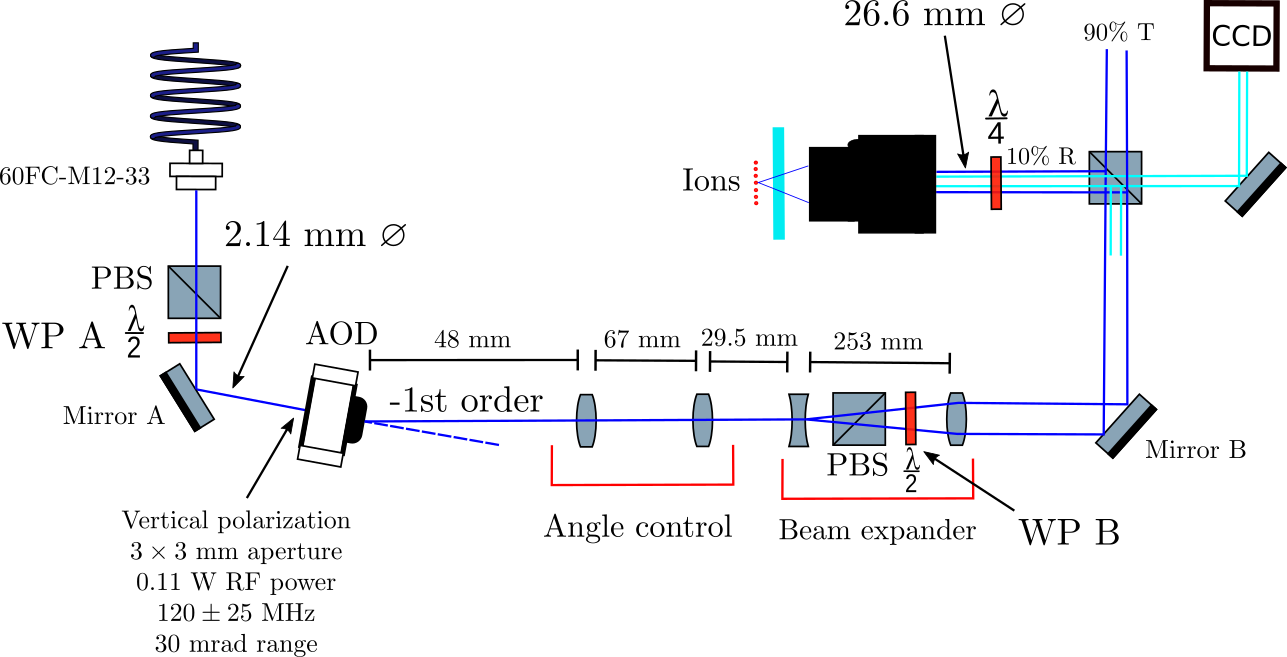
\includegraphics[width=\textwidth]{img/setup}
\caption{Setup scheme}
\end{figure}


\begin{figure}[H]
\centering
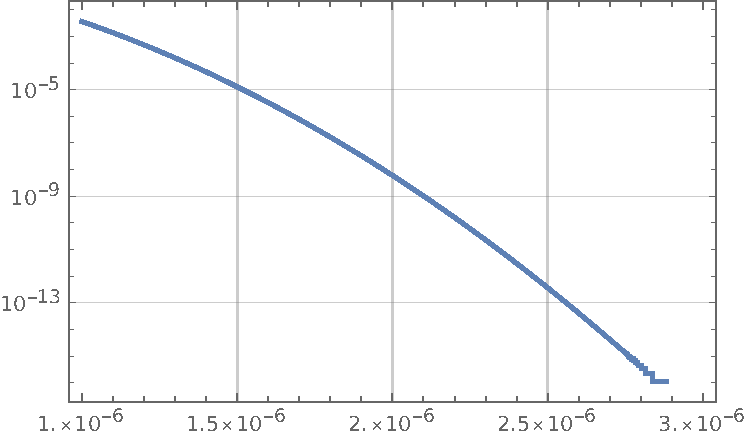
\includegraphics[width=\textwidth]{img/Plosses}
\caption{Losses on the compensation electrodes vs beam waist}
\end{figure}
\begin{figure}[H]
\centering
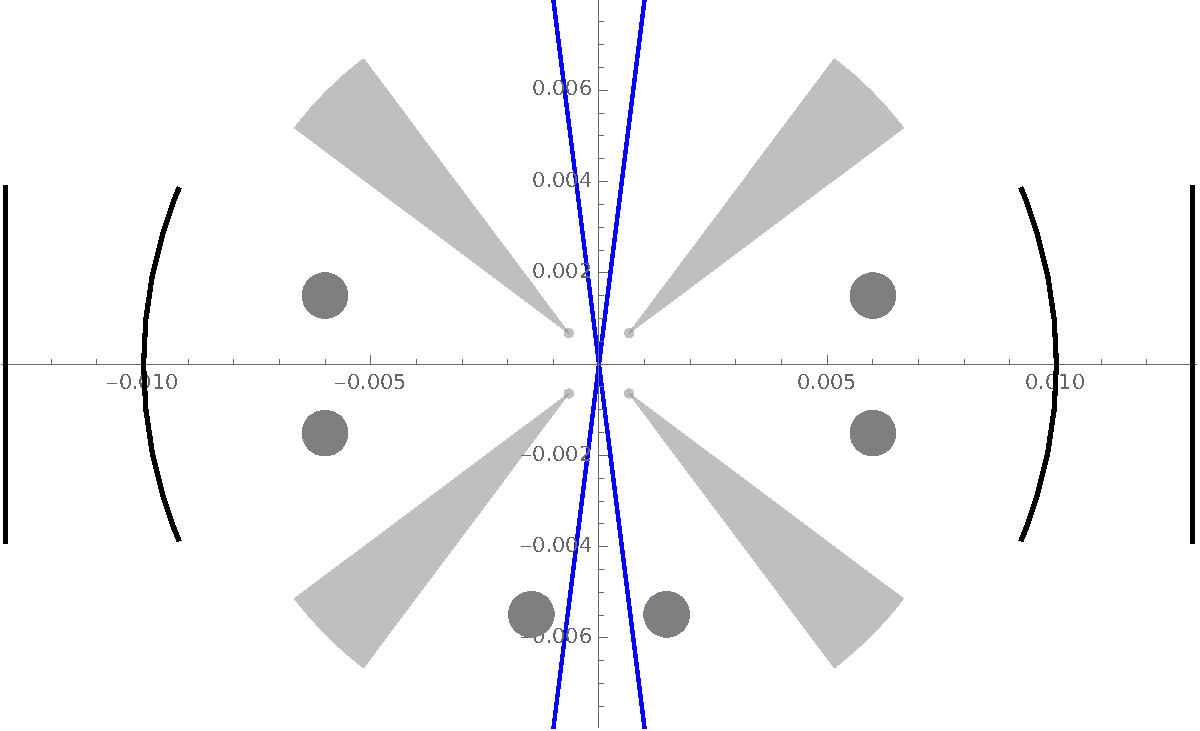
\includegraphics[width=\textwidth]{img/clipping}
\caption{Clipping on compensation electrodes}
\end{figure}

\chapter{Existing experimental system}
\section{Ion trap and key techniques}
\subsection{Calcium Ions}
- Calcium level scheme basically
\subsection{Trapping, cooling, and state readout}
- How this stuff is implemented
\subsection{Photon generations}
- Cavity enhanced Raman transition
\section{393nm laser}
\section{Experiment control}
\chapter{Design and simulation of the addressing setup}
\section{Addressing system overview and requirements}
\section{Objective and AOD}
\section{Addressing setup}
- Scheme of real setup \\
- Alignment process

\chapter{Experimental results}
\section{AOD}
\section{Full test setup characterisation}
\subsection{Test: razor blade and camera}
\begin{figure}[H]
\centering
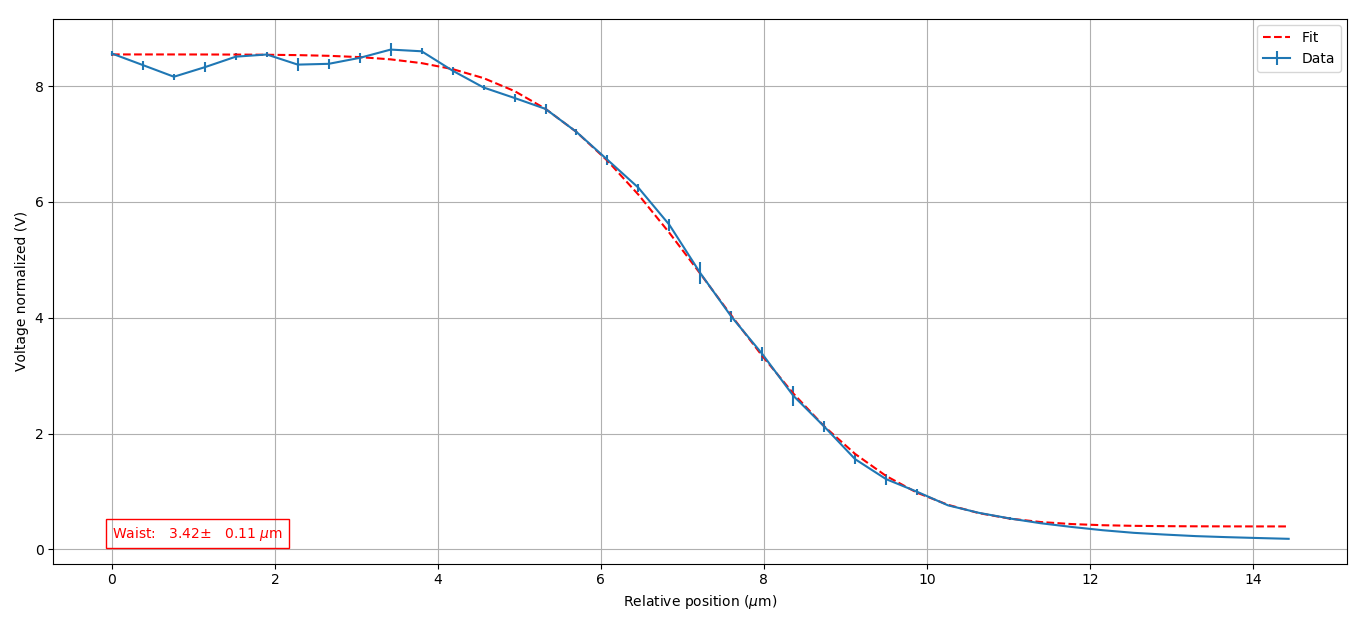
\includegraphics[width=\textwidth]{img/prova7}
\caption{Example of razor scan}
\end{figure}
\begin{figure}[H]
\centering
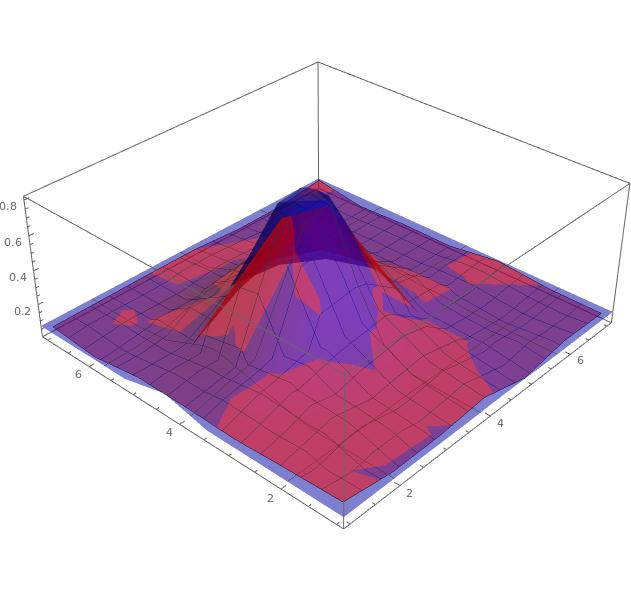
\includegraphics[width=\textwidth]{img/camera}
\caption{Example of camera picture}
\end{figure}
\subsection{Polarization characterization}
\subsection{Stability}
\section{Final installed system}
\subsection{Ramsey interferometry}
\begin{figure}[H]
\centering
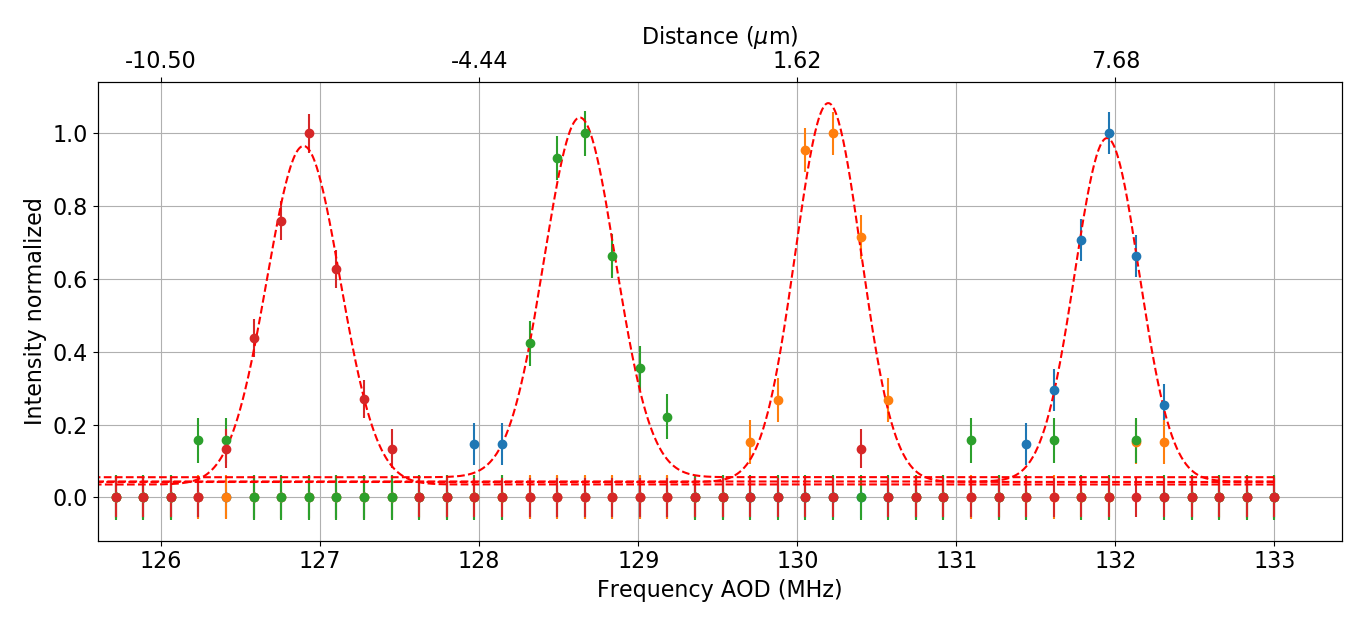
\includegraphics[width=\textwidth]{img/AODscan}
\caption{3 ions scanned}
\end{figure}
\begin{figure}[H]
\centering
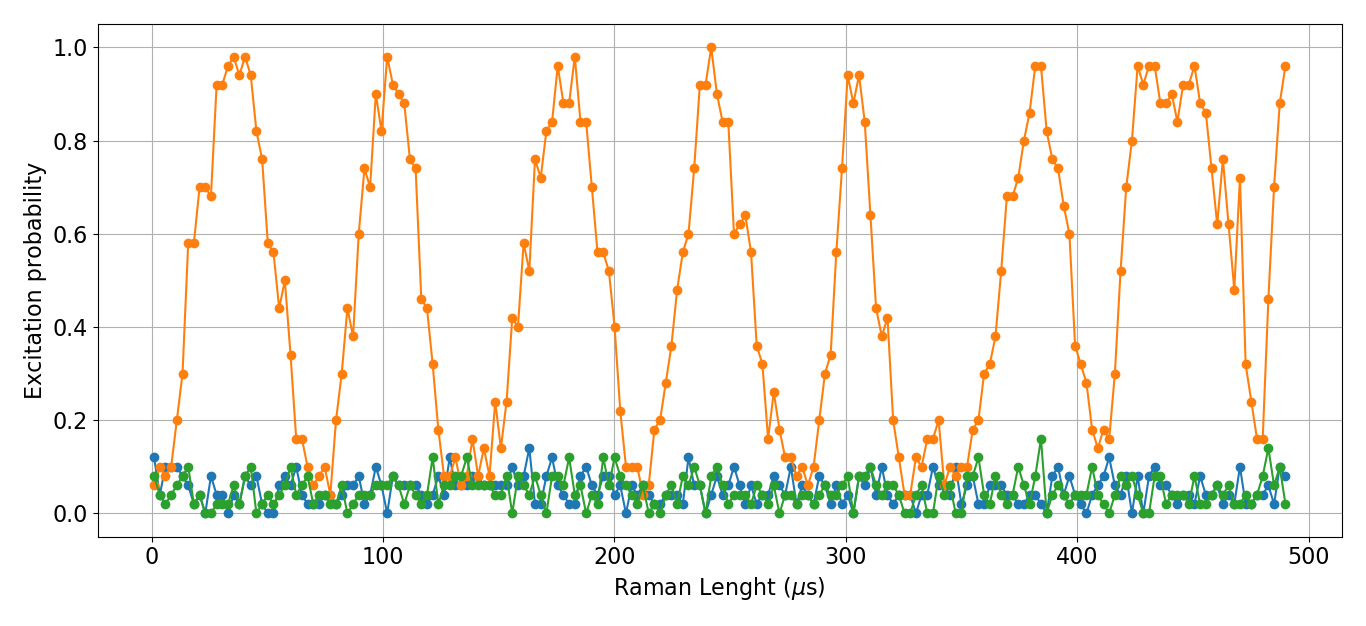
\includegraphics[width=\textwidth]{img/ac_stark}
\caption{393nm AC-Stark flops}
\end{figure}

\subsection{Photons production}
\begin{figure}[H]
\centering
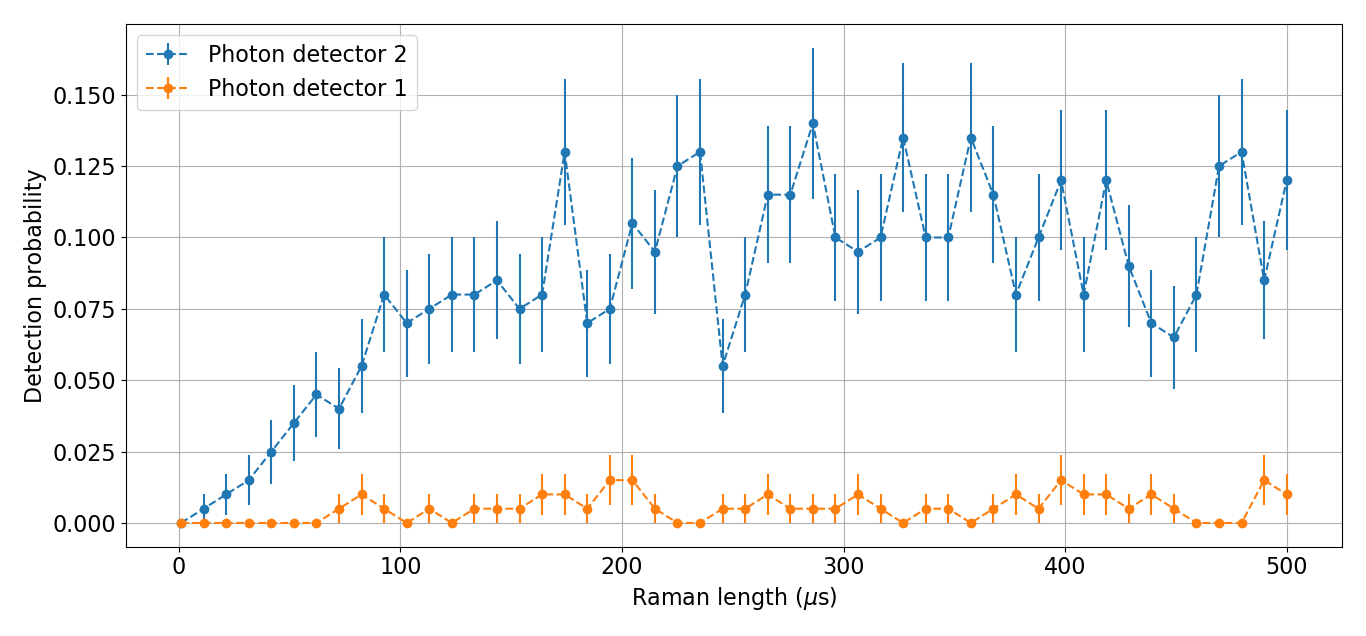
\includegraphics[width=\textwidth]{img/photonefficency_witherror}
\caption{Generated photon efficency}
\end{figure}

\begin{figure}[H]
\centering
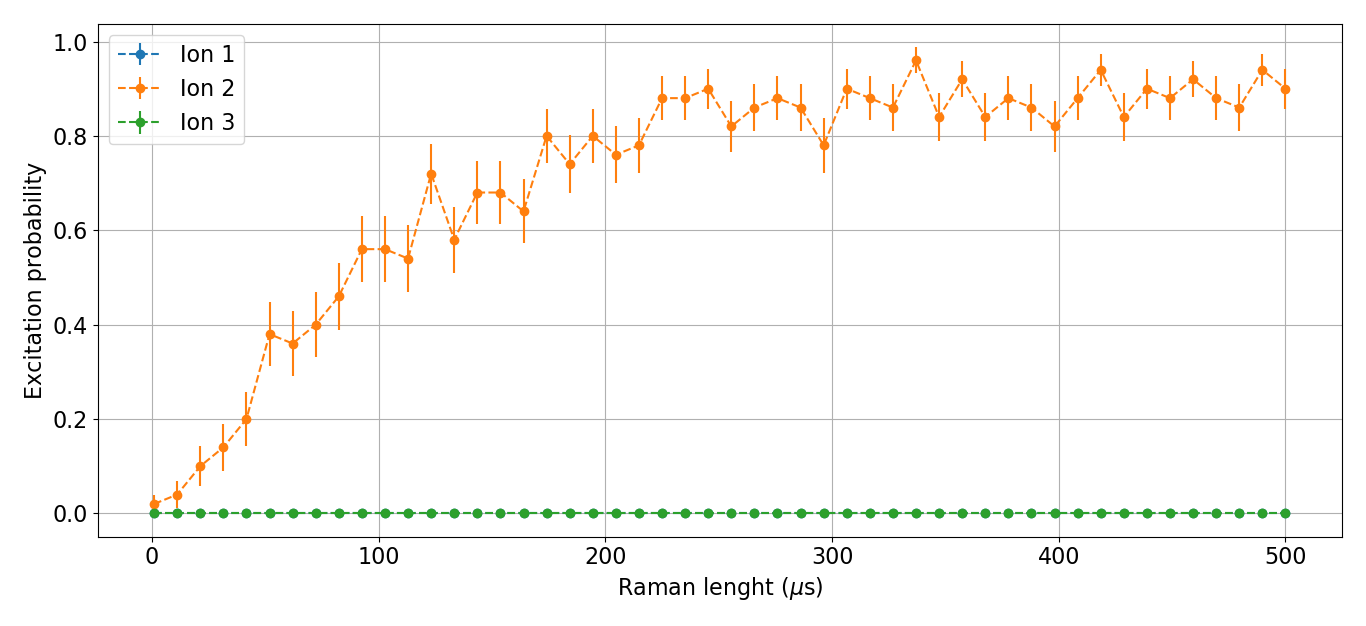
\includegraphics[width=\textwidth]{img/ramanlength_witherrors}
\caption{Excitation of ion while emitting photon}
\end{figure}

- g2 plot?
\section{Final properties summary}

\chapter{Conclusions and outlook}
- Usual conclusions

\newpage
%\renewcommand\refname{References} % name for the reference list

\addcontentsline{toc}{section}{References} % to change the name of the references in the TOC
\bibliographystyle{plain}
\bibliography{References} % adds the references to the document


\newpage
\renewcommand{\appendixpagename}{Appendix} % Heading of appendix
\renewcommand{\appendixtocname}{Appendix} % name of appendix in TOC
\appendixpage
\addappheadtotoc


\begin{appendices}
- Error analysis? Maximum likehood estimation?
\end{appendices}

\end{document}
